\chapter{Cell tracking results}
	\label{app:appendix_trackingresults}
	
	This chapter includes three-dimensional figures of the trajectories generated by the cell tracking module on four of the studied datasets.

\begin{figure}[h]
	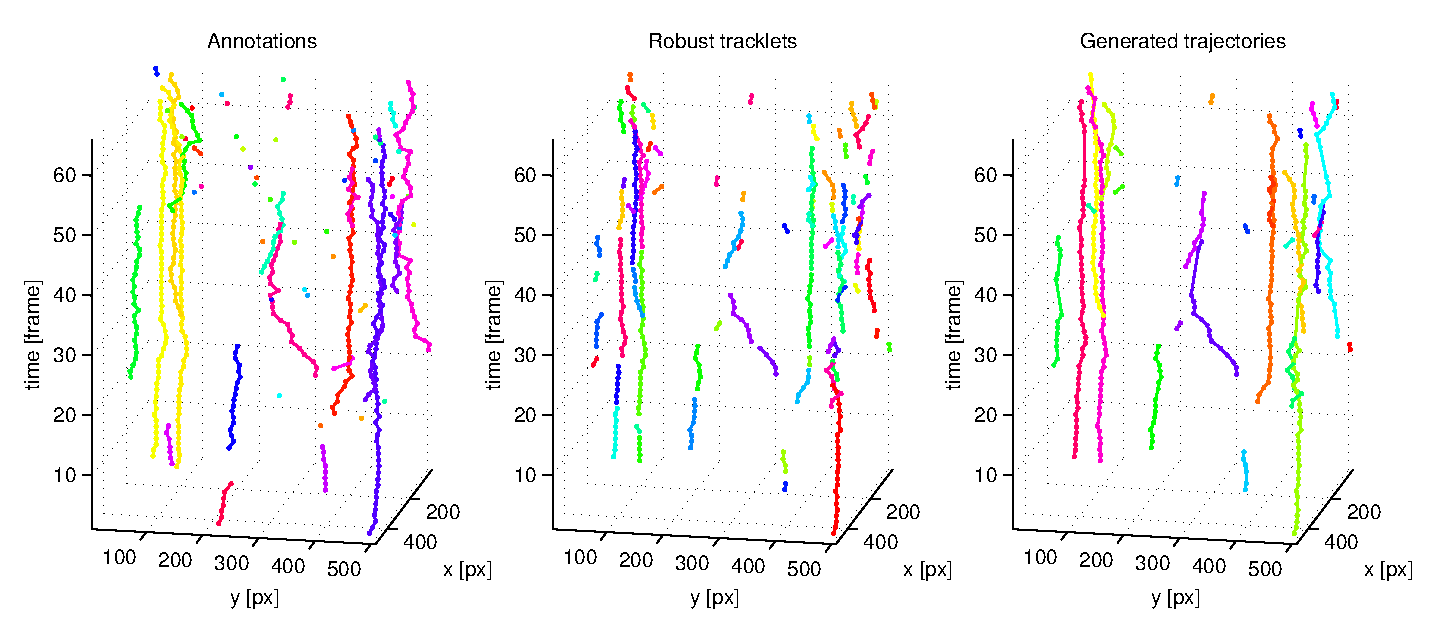
\includegraphics[width=\textwidth]{images/fig_results_tracker_dataset_2}
	\caption{Generated trajectories for dataset B. The parameters of the tracker were set to $\pi_{init}=1$, $\pi_{term}=1$, $\pi_{link}=1$ and $\pi_{FP}=1$ and configured to close gaps up to size 9.}
	\label{fig:results_tracker_dataset_2}
\end{figure}


\begin{figure}[h]
	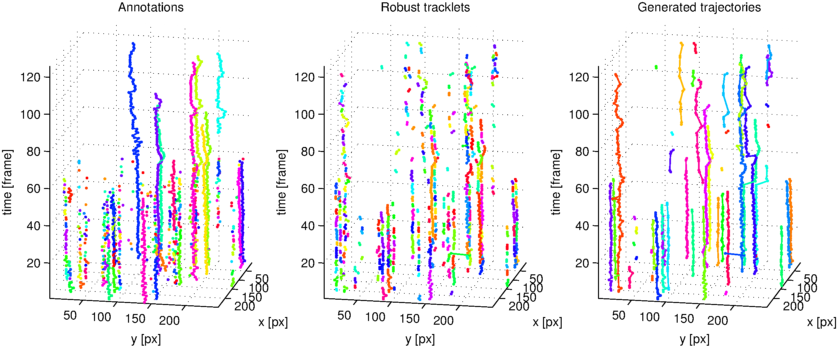
\includegraphics[width=\textwidth]{images/fig_results_tracker_dataset_3}
	\caption{Generated trajectories for dataset C. The parameters of the tracker were set to $\pi_{init}=1$, $\pi_{term}=1$, $\pi_{link}=1$ and $\pi_{FP}=1$ and configured to close gaps up to size 9.}
	\label{fig:results_tracker_dataset_3}
\end{figure}

\begin{figure}[h]
	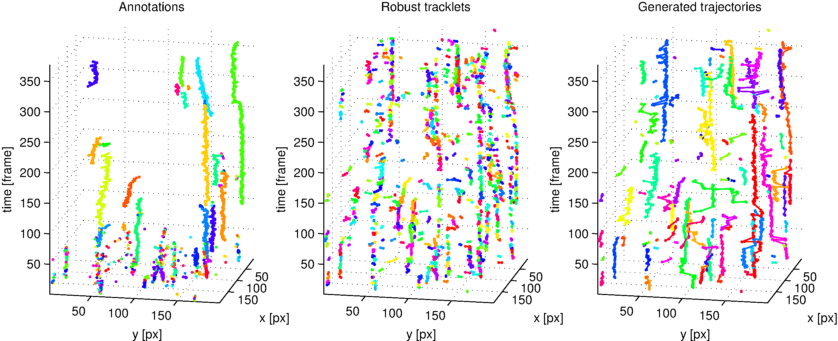
\includegraphics[width=\textwidth]{images/fig_results_tracker_dataset_4}
	\caption{Generated trajectories for dataset D. The parameters of the tracker were set to $\pi_{init}=1$, $\pi_{term}=1$, $\pi_{link}=1$ and $\pi_{FP}=1$ and configured to close gaps up to size 9. }
	\label{fig:results_tracker_dataset_4}
\end{figure}
\begin{figure}[h]
	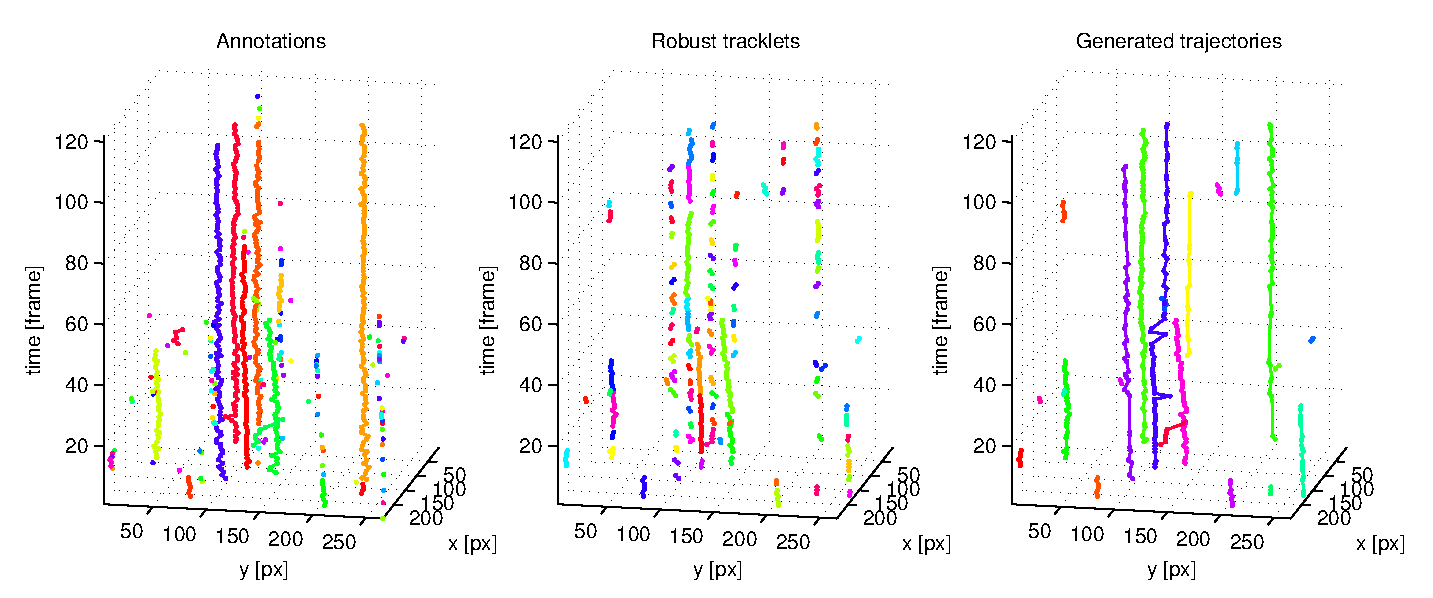
\includegraphics[width=\textwidth]{images/fig_results_tracker_dataset_5}
	\caption{Generated trajectories for dataset E. The parameters of the tracker were set to $\pi_{init}=3$, $\pi_{term}=3$, $\pi_{link}=1$ and $\pi_{FP}=1$ and configured to close gaps iteratively up to size 9 and then up to size 20.}
	\label{fig:results_tracker_dataset_5}
\end{figure}			